%
% $Id: slides.tex 4228 2006-06-21 21:55:12Z jjamor $
%
%
% Compilar a .pdf con LaTeX (pdflatex)
% Es necesario instalar Beamer (paquete latex-beamer en Debian)
%

%
% Gráficos:
% Los gráficos pueden suministrarse en PNG, JPG, TIF, PDF, MPS
% Los EPS deben convertirse a PDF (usar epstopdf)
%

\documentclass{beamer}
\usetheme{Warsaw}
\usebackgroundtemplate{
\includegraphics[width=\paperwidth]{format/libresoft-bg.png}}
\usepackage[spanish]{babel}
\usepackage[utf8]{inputenc}
\usepackage{graphics}
\usepackage{amssymb} % Simbolos matematicos
\usepackage{url}

%\definecolor{libresoftgreen}{RGB}{162,190,43}
%\definecolor{libresoftblue}{RGB}{0,98,143}

%\setbeamercolor{titlelike}{bg=libresoftgreen}

%% Metadatos del PDF.
\hypersetup{
  pdftitle={The Onion Model in FLOSS},
  pdfauthor={F. Ortega, J.J. Amor, G. Robles},
  pdfcreator={GSyC/Libresoft},
  pdfproducer=PDFLaTeX,
  pdfsubject={nn},
}
%%


\AtBeginSection[]
{
  \begin{frame}<presentation>
    \frametitle{Index}
    \tableofcontents[current]
  \end{frame}
}


\begin{document}

\title{The Onion Model in FLOSS}
\subtitle{Master on Free Software}
\institute{\\jfelipe@libresoft.es\\
GSyC/Libresoft}
\author{Felipe Ortega, Juan José Amor, Gregorio Robles}
\date{\today}

\frame{
\maketitle
\begin{center}

\includegraphics[width=6cm]{format/gsyc-urjc}
\end{center}
}


% Si el titulo o el autor se quieren acortar para los pies de p�gina
% se pueden redefinir aqu�:
%\title{Titulo corto}
%\author{Autores abreviado}


%% LICENCIA DE REDISTRIBUCION DE LAS TRANSPAS
\frame{
~
\vspace{4cm}

\begin{flushright}
{\tiny
(cc) 2007-2010 Felipe Ortega, Juanjo Amor, Gregorio Robles. \\
Some rights reserved. This document is distributed under the Creative \\
            Commons Attribution-ShareAlike 3.0 licence, available in \\
            http://creativecommons.org/licenses/by-sa/3.0/

%  Este documento (o uno muy similar) está disponible en \\
%  \url{http://gsyc.escet.urjc.es/~jjamor/}
}
\end{flushright}
}
%%

%%%%%%
%Transpas separadas por \begin{frame}
%%%%%%%%%%%%%%%%%%%%%%%%\end{frame}

\section{Introduction}

\begin{frame}
\frametitle{Why studying FLOSS social structure?}
\begin{itemize}
\item Describe and account advantages of FLOSS organization
\item Characterize communication patterns in FLOSS project.
\item Can we find out common structures in FLOSS projects?
\end{itemize}
\end{frame}

%%%%%%%%%%%%%%%%%%%%%%%%%%%%%%%%%%%%%%%%%%%%%%%%%%%%%%%%%%%%%%

\begin{frame}
 \frametitle{Overview of the analysis}
 \begin{itemize}
 \item Crowston \& Howison examined 120 project teams from
SourceForge.
 \item They focus on communications centralization (BTS).
 \item They find wide variations in centralization degree.
 \item But they also find a common stratification pattern:
  \textbf{the onion model}
 \end{itemize}
\end{frame}

%%%%%%%%%%%%%%%%%%%%%%%%%%%%%%%%%%%%%%%%%%%%%%%%%%%%%%%%%%%%%%

\section{Social structure of FLOSS projects}

%%%%%%%%%%%%%%%%%%%%%%%%%%%%%%%%%%%%%%%%%%%%%%%%%%%%%%%%%%%%%%

\begin{frame}
\frametitle{Social Structure of FLOSS projects}
\begin{center}
\begin{figure}
 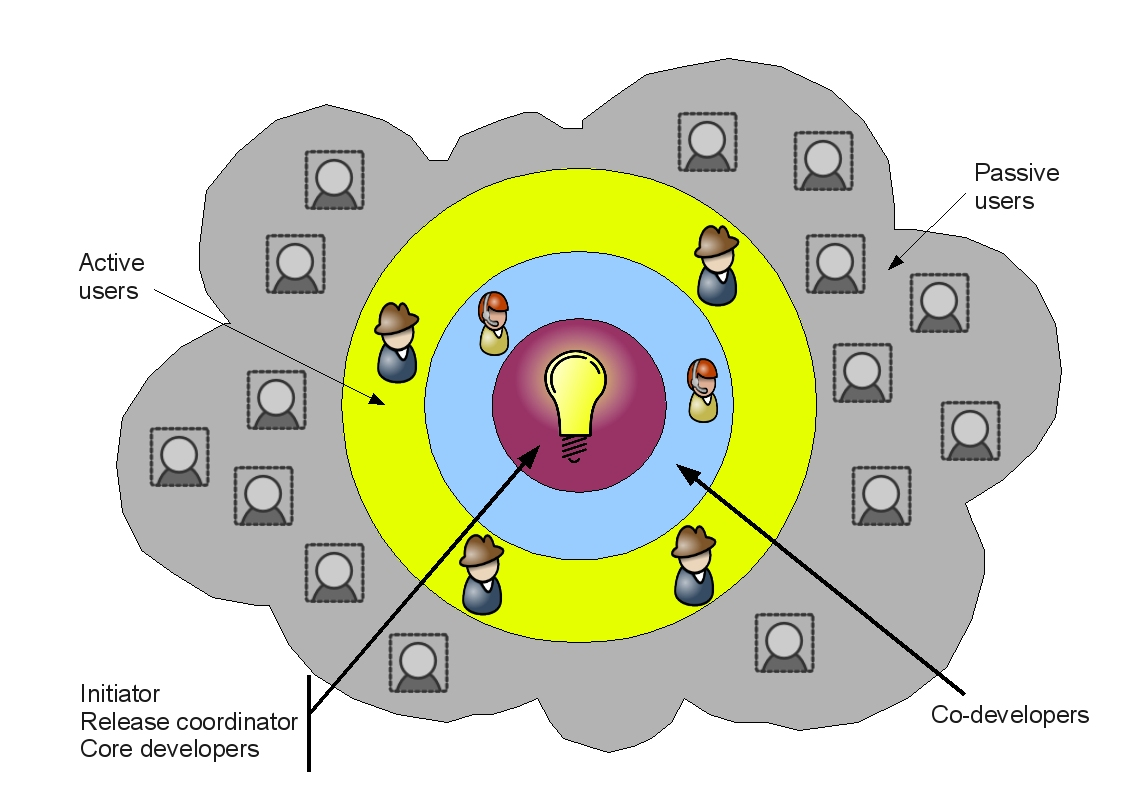
\includegraphics[height=7.5cm]{figs/onion-model.jpg}
\end{figure}
\end{center}
\end{frame}

%%%%%%%%%%%%%%%%%%%%%%%%%%%%%%%%%%%%%%%%%%%%%%%%%%%%%%%%%%%%%%

\begin{frame}
 \frametitle{Other analyses of social structure in FLOSS}
 \begin{itemize}
  \item Apache \textbf{httpd} (Mockus \emph{et al.}, 2000)
  \begin{itemize}
   \item Only 15 developers contributing more than 80 percent
   of the code.
   \item Usual example of Pareto's Law.
   \item Size of each layer differs by an order of magnitude
    \item \begin{footnotesize}[Mockus 2000] A. Mockus et al, ``A case study of open source software development:
      the Apache server'' (2000)
      \url{http://opensource.mit.edu/papers/mockusapache.pdf}\end{footnotesize}
  \end{itemize}
  \item Debian (Robles \emph{et al.} 2006, Michlmayr \emph{et al.} 2005)
  \begin{itemize}
   \item The composition of the core evolves over time.
   \item Half-life ratio: 7.5 years
  \end{itemize}
 \end{itemize}
\end{frame}

%%%%%%%%%%%%%%%%%%%%%%%%%%%%%%%%%%%%%%%%%%%%%%%%%%%%%%%%%%%%%%

\begin{frame}
\frametitle{Evolution of FLOSS projects}
\begin{center}
\begin{figure}
 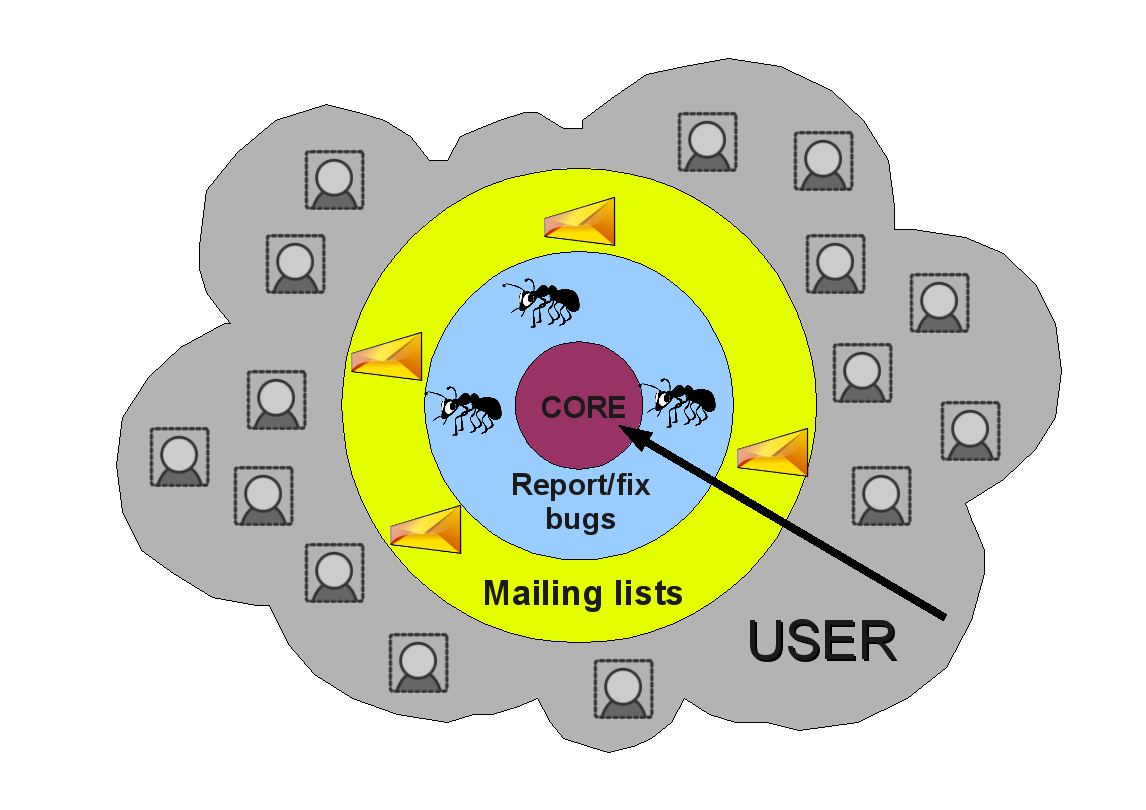
\includegraphics[height=7.5cm]{figs/progression.png}
\end{figure}
\end{center}
\end{frame}

%%%%%%%%%%%%%%%%%%%%%%%%%%%%%%%%%%%%%%%%%%%%%%%%%%%%%%%%%%%%%%

\begin{frame}
\frametitle{Evolution of the ``core'' group}

\begin{center}
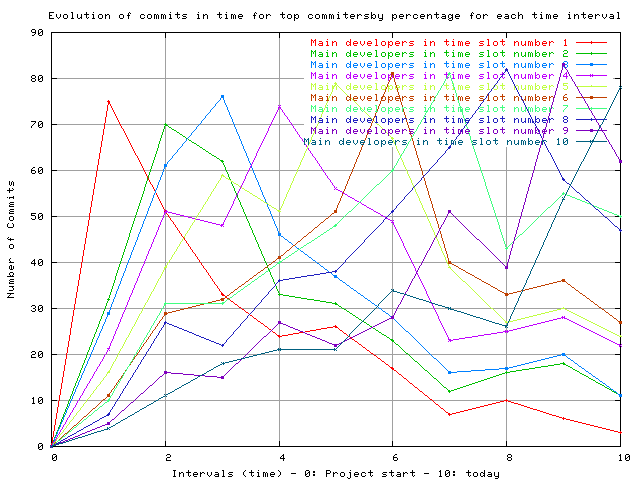
\includegraphics[height=6.5cm]{figs/mozilla_log-per_10_22.png}
\end{center}

\end{frame}

%%%%%%%%%%%%%%%%%%%%%%%%%%%%%%%%%%%%%%%%%%%%%%%%%%%%%%%%%%%%%%

\begin{frame}
\frametitle{Social Network Analysis (I)}

\begin{center}
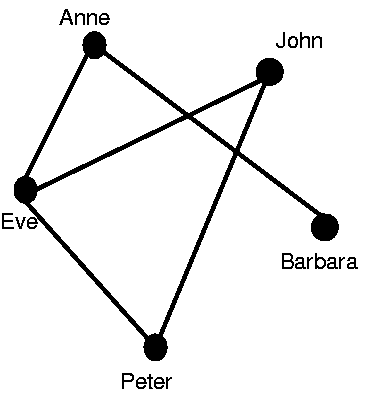
\includegraphics[width=6cm]{figs/simple-sna.png}
\end{center}

\end{frame}

%%%%%%%%%%%%%%%%%%%%%%%%%%%%%%%%%%%%%%%%%%%%%%%%%%%%%%%%%%%%%%

\begin{frame}
\frametitle{Social Network Analysis (II)}

\begin{center}
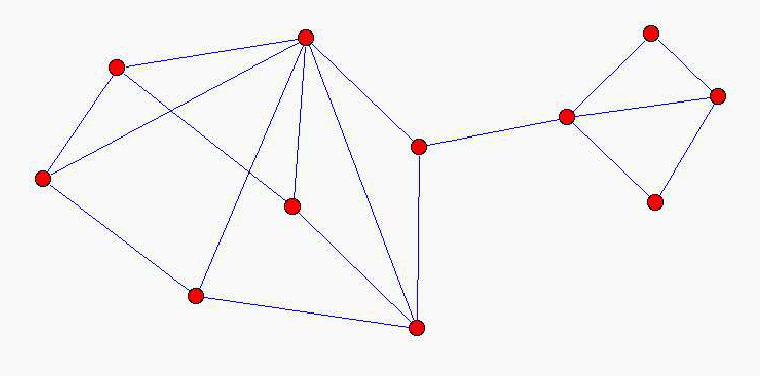
\includegraphics[width=9cm]{figs/sna-one.png}
\end{center}

\end{frame}

%%%%%%%%%%%%%%%%%%%%%%%%%%%%%%%%%%%%%%%%%%%%%%%%%%%%%%%%%%%%%%

\begin{frame}
\frametitle{Social Network Analysis (and III)}

\begin{center}
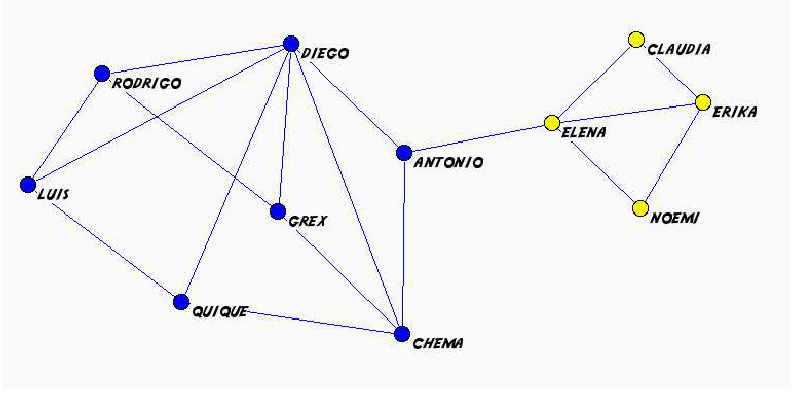
\includegraphics[width=11cm]{figs/sna-two.png}
\end{center}

\end{frame}

%%%%%%%%%%%%%%%%%%%%%%%%%%%%%%%%%%%%%%%%%%%%%%%%%%%%%%%%%%%%%%

\begin{frame}
\frametitle{SNA for Linux 1.0}

\begin{center}
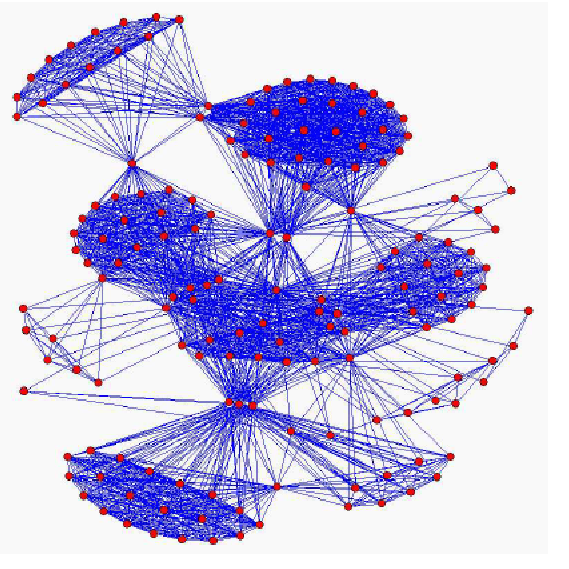
\includegraphics[width=7cm]{figs/linux1-sna.png}
\end{center}

\end{frame}

%%%%%%%%%%%%%%%%%%%%%%%%%%%%%%%%%%%%%%%%%%%%%%%%%%%%%%%%%%%%%%

\begin{frame}
\frametitle{Developer Territoriality}

\begin{center}
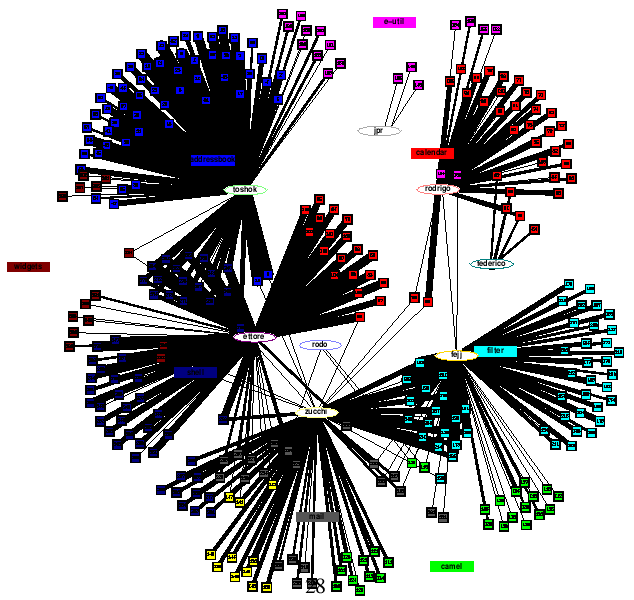
\includegraphics[width=7cm]{figs/german-territoriality.png}
\end{center}

\end{frame}

%%%%%%%%%%%%%%%%%%%%%%%%%%%%%%%%%%%%%%%%%%%%%%%%%%%%%%%%%%%%%%

\section{Practice: analysis of \bfseries{brasero}}

%%%%%%%%%%%%%%%%%%%%%%%%%%%%%%%%%%%%%%%%%%%%%%%%%%%%%%%%%%%%%%

\begin{frame}
\frametitle{Proposed practice}
 \begin{itemize}
  \item Load \textbf{brasero} data set from FLOSSMetrics DB.
  \item Activities:
  \begin{enumerate}
   \item Identify the most active contributor, and the top 20 contributors.
   \item Plot a graph diplaying the differences in the number of contributions.
   \texttt{barplot()}.\\Hint use \textbf{scmlog} table in \textbf{fm3\_evince\_svn\_scm}.
   \item Identify changes in the most active contributor (every year).\\
   \item Each layer should be an order of magnitude larger than the
   previous one. How many layers do we have?
  \end{enumerate}
  \item Homework: Analyze bug tracking system, searching for evidences
  of different onion-like layers.
 \end{itemize}
\end{frame}

%%%%%%%%%%%%%%%%%%%%%%%%%%%%%%%%%%%%%%%%%%%%%%%%%%%%%%%%%%%%%%

\begin{frame}[fragile]
\frametitle{Some hints for the practice (I)}
\begin{itemize}
\item Download CVSAnalY archives\\
\item Source: \url{http://melquiades.flossmetrics.org}
 \begin{verbatim}
$ gunzip fm3_brasero_cvsanaly2_svn_scm...sql.gz
$ gunzip fm3_brasero_bicho_bg_trk_...sql.gz
\end{verbatim}
\item Create DB (only for fm3\_brasero\_bicho) in MySQL:
\begin{verbatim}
$ mysql -u myuser -pmypassw < fm3_cvsanaly2_...sql
$ mysql -u myuser -pmypassw \
fm3_brasero_bicho < fm3_brasero_bicho_bg_trk_...sql
 \end{verbatim}
\end{itemize}
\end{frame}

%%%%%%%%%%%%%%%%%%%%%%%%%%%%%%%%%%%%%%%%%%%%%%%%%%%%%%%%%%%%%%

\begin{frame}[fragile]
\frametitle{Some hints for the practice (II)}

\begin{itemize}
 \item Access MySQL DBs from GNU R.
\end{itemize}
\vspace{-0.5cm}
\begin{verbatim}
 > library(RMySQL)
 > con <- dbConnect(MySQL(), u="phoenix", p="secret",
 db="fm3_brasero_svn_scm") #Open DB connection
 > dbListTables(con)
 > dbListFields(con, "table_name")
 > #Execute query, store results in a data frame
 > df = dbGetQuery(con, "select * from table_name") 
 > dbDisconnect(con) #Close DB connection
 > ?RMySQL # more examples
\end{verbatim}

\end{frame}

%%%%%%%%%%%%%%%%%%%%%%%%%%%%%%%%%%%%%%%%%%%%%%%%%%%%%%%%%%%%%%

\begin{frame}[fragile]
\frametitle{Some hints for the practice (III)}
\begin{itemize}
\item Some R functions you may want to use:
  \begin{itemize}
  \item \texttt{summary(df)}
  \item \texttt{plot(df\$x,df\$y, type=''b'', colour=''navy'',...)}
  \item \texttt{barplot(df\$y, names.arg=df\$x, colour=''olive'',...)}
  \item \texttt{boxplot(df\$x)}
  \item \texttt{histogram(df\$x); lines(density(df\$x))}
  \end{itemize}
\end{itemize}
\end{frame}
\end{document}